%% Beginning of file 'sample631.tex'
%%
%% Modified 2021 March
%%
%% This is a sample manuscript marked up using the
%% AASTeX v6.31 LaTeX 2e macros.
%%
%% AASTeX is now based on Alexey Vikhlinin's emulateapj.cls 
%% (Copyright 2000-2015).  See the classfile for details.

%% AASTeX requires revtex4-1.cls and other external packages such as
%% latexsym, graphicx, amssymb, longtable, and epsf.  Note that as of 
%% Oct 2020, APS now uses revtex4.2e for its journals but remember that 
%% AASTeX v6+ still uses v4.1. All of these external packages should 
%% already be present in the modern TeX distributions but not always.
%% For example, revtex4.1 seems to be missing in the linux version of
%% TexLive 2020. One should be able to get all packages from www.ctan.org.
%% In particular, revtex v4.1 can be found at 
%% https://www.ctan.org/pkg/revtex4-1.

%% The first piece of markup in an AASTeX v6.x document is the \documentclass
%% command. LaTeX will ignore any data that comes before this command. The 
%% documentclass can take an optional argument to modify the output style.
%% The command below calls the preprint style which will produce a tightly 
%% typeset, one-column, single-spaced document.  It is the default and thus
%% does not need to be explicitly stated.
%%
%% using aastex version 6.3
\documentclass[linenumbers,modern,astrosymb,times]{aastex631dm}

%% The default is a single spaced, 10 point font, single spaced article.
%% There are 5 other style options available via an optional argument. They
%% can be invoked like this:
%%
%% \documentclass[arguments]{aastex631}
%% 
%% where the layout options are:
%%
%%  twocolumn   : two text columns, 10 point font, single spaced article.
%%                This is the most compact and represent the final published
%%                derived PDF copy of the accepted manuscript from the
%%                publisher
%%  manuscript  : one text column, 12 point font, double spaced article.
%%  preprint    : one text column, 12 point font, single spaced article.  
%%  preprint2   : two text columns, 12 point font, single spaced article.
%%  modern      : a stylish, single text column, 12 point font, article with
%% 		  wider left and right margins. This uses the Daniel
%% 		  Foreman-Mackey and David Hogg design.
%%  RNAAS       : Supresses an abstract. Originally for RNAAS manuscripts 
%%                but now that abstracts are required this is obsolete for
%%                AAS Journals. Authors might need it for other reasons. DO NOT
%%                use \begin{abstract} and \end{abstract} with this style.
%%
%% Note that you can submit to the AAS Journals in any of these 6 styles.
%%
%% There are other optional arguments one can invoke to allow other stylistic
%% actions. The available options are:
%%
%%   astrosymb    : Loads Astrosymb font and define \astrocommands. 
%%   tighten      : Makes baselineskip slightly smaller, only works with 
%%                  the twocolumn substyle.
%%   times        : uses times font instead of the default
%%   linenumbers  : turn on lineno package.
%%   trackchanges : required to see the revision mark up and print its output
%%   longauthor   : Do not use the more compressed footnote style (default) for 
%%                  the author/collaboration/affiliations. Instead print all
%%                  affiliation information after each name. Creates a much 
%%                  longer author list but may be desirable for short 
%%                  author papers.
%% twocolappendix : make 2 column appendix.
%%   anonymous    : Do not show the authors, affiliations and acknowledgments 
%%                  for dual anonymous review.
%%
%% these can be used in any combination, e.g.
%%
%% \documentclass[twocolumn,linenumbers,trackchanges]{aastex631}
%%
%% AASTeX v6.* now includes \hyperref support. While we have built in specific
%% defaults into the classfile you can manually override them with the
%% \hypersetup command. For example,
%%
%% \hypersetup{linkcolor=red,citecolor=green,filecolor=cyan,urlcolor=magenta}
%%
%% will change the color of the internal links to red, the links to the
%% bibliography to green, the file links to cyan, and the external links to
%% magenta. Additional information on \hyperref options can be found here:
%% https://www.tug.org/applications/hyperref/manual.html#x1-40003
%%
%% Note that in v6.3 "bookmarks" has been changed to "true" in hyperref
%% to improve the accessibility of the compiled pdf file.
%%

%% Relax deluxtable's \tablenum command to allow siunitx to overwrite it
\let\tablenum\relax  % Use \savetablenum instead with deluxtable

\usepackage{siunitx}
    \sisetup{
        separate-uncertainty,
        range-units=single,
        multi-part-units=single
    }

\usepackage{bm}
\usepackage{amsmath,amssymb}

%% Colors
\definecolor{todo}{rgb}{0.9, 0.1, 0.1}
\definecolor{comment}{rgb}{0.2, 0.7, 0.3}

%% If you want to create your own macros, you can do so
%% using \newcommand. Your macros should appear before
%% the \begin{document} command.
%%
%% Text commands
\newcommand{\aastex}{AAS\TeX}
\newcommand{\latex}{La\TeX}

%% Math commands
\newcommand{\vdag}{(v)^\dagger}
\newcommand{\helium}{\mathrm{He}}
\newcommand{\bcz}{\mathrm{BCZ}}
\newcommand{\bkg}{\mathrm{bkg}}
\newcommand{\npred}{n_{\star}}
\newcommand{\dd}{\mathrm{d}}

%% In-text annotation commands
\newcommand{\todo}[1]{{\color{todo} \textbf{TODO:} #1}}
\newcommand{\comment}[2]{{\color{comment} \textbf{#1:} #2}}
\newcommand{\needcite}{\todo{citation needed}}

%% Define figure width as a fraction of line width
\ifmodern
\newcommand{\figscale}{0.86}
\else
\newcommand{\figscale}{1.0}
\fi

%% Reintroduced the \received and \accepted commands from AASTeX v5.2
%\received{March 1, 2021}
%\revised{April 1, 2021}
%\accepted{\today}

%% Command to document which AAS Journal the manuscript was submitted to.
%% Adds "Submitted to " the argument.
%\submitjournal{PSJ}

%% For manuscript that include authors in collaborations, AASTeX v6.31
%% builds on the \collaboration command to allow greater freedom to 
%% keep the traditional author+affiliation information but only show
%% subsets. The \collaboration command now must appear AFTER the group
%% of authors in the collaboration and it takes TWO arguments. The last
%% is still the collaboration identifier. The text given in this
%% argument is what will be shown in the manuscript. The first argument
%% is the number of author above the \collaboration command to show with
%% the collaboration text. If there are authors that are not part of any
%% collaboration the \nocollaboration command is used. This command takes
%% one argument which is also the number of authors above to show. A
%% dashed line is shown to indicate no collaboration. This example manuscript
%% shows how these commands work to display specific set of authors 
%% on the front page.
%%
%% For manuscript without any need to use \collaboration the 
%% \AuthorCollaborationLimit command from v6.2 can still be used to 
%% show a subset of authors.
%
%\AuthorCollaborationLimit=2
%
%% will only show Schwarz & Muench on the front page of the manuscript
%% (assuming the \collaboration and \nocollaboration commands are
%% commented out).
%%
%% Note that all of the author will be shown in the published article.
%% This feature is meant to be used prior to acceptance to make the
%% front end of a long author article more manageable. Please do not use
%% this functionality for manuscripts with less than 20 authors. Conversely,
%% please do use this when the number of authors exceeds 40.
%%
%% Use \allauthors at the manuscript end to show the full author list.
%% This command should only be used with \AuthorCollaborationLimit is used.

%% The following command can be used to set the latex table counters.  It
%% is needed in this document because it uses a mix of latex tabular and
%% AASTeX deluxetables.  In general it should not be needed.
%\setcounter{table}{1}

%%%%%%%%%%%%%%%%%%%%%%%%%%%%%%%%%%%%%%%%%%%%%%%%%%%%%%%%%%%%%%%%%%%%%%%%%%%%%%%
%%
%% The following section outlines numerous optional output that
%% can be displayed in the front matter or as running meta-data.
%%
%% If you wish, you may supply running head information, although
%% this information may be modified by the editorial offices.
\shorttitle{Acoustic glitches in solar-like oscillators}
\shortauthors{Lyttle et al.}
%%
%% You can add a light gray and diagonal water-mark to the first page 
%% with this command:
\watermark{DRAFT}
%% where "text", e.g. DRAFT, is the text to appear.  If the text is 
%% long you can control the water-mark size with:
%% \setwatermarkfontsize{dimension}
%% where dimension is any recognized LaTeX dimension, e.g. pt, in, etc.
%%
%%%%%%%%%%%%%%%%%%%%%%%%%%%%%%%%%%%%%%%%%%%%%%%%%%%%%%%%%%%%%%%%%%%%%%%%%%%%%%%
\ifdarkmode
\graphicspath{{./}{figures-dm/}}
\else
\graphicspath{{./}{figures/}}
\fi
%% This is the end of the preamble.  Indicate the beginning of the
%% manuscript itself with \begin{document}.

\begin{document}

\title{
    Measuring acoustic glitches in the modes of solar-like oscillators
    using Gaussian processes
}

%% LaTeX will automatically break titles if they run longer than
%% one line. However, you may use \\ to force a line break if
%% you desire. In v6.31 you can include a footnote in the title.

%% A significant change from earlier AASTEX versions is in the structure for 
%% calling author and affiliations. The change was necessary to implement 
%% auto-indexing of affiliations which prior was a manual process that could 
%% easily be tedious in large author manuscripts.
%%
%% The \author command is the same as before except it now takes an optional
%% argument which is the 16 digit ORCID. The syntax is:
%% \author[xxxx-xxxx-xxxx-xxxx]{Author Name}
%%
%% This will hyperlink the author name to the author's ORCID page. Note that
%% during compilation, LaTeX will do some limited checking of the format of
%% the ID to make sure it is valid. If the "orcid-ID.png" image file is 
%% present or in the LaTeX pathway, the OrcID icon will appear next to
%% the authors name.
%%
%% Use \affiliation for affiliation information. The old \affil is now aliased
%% to \affiliation. AASTeX v6.31 will automatically index these in the header.
%% When a duplicate is found its index will be the same as its previous entry.
%%
%% Note that \altaffilmark and \altaffiltext have been removed and thus 
%% can not be used to document secondary affiliations. If they are used latex
%% will issue a specific error message and quit. Please use multiple 
%% \affiliation calls for to document more than one affiliation.
%%
%% The new \altaffiliation can be used to indicate some secondary information
%% such as fellowships. This command produces a non-numeric footnote that is
%% set away from the numeric \affiliation footnotes.  NOTE that if an
%% \altaffiliation command is used it must come BEFORE the \affiliation call,
%% right after the \author command, in order to place the footnotes in
%% the proper location.
%%
%% Use \email to set provide email addresses. Each \email will appear on its
%% own line so you can put multiple email address in one \email call. A new
%% \correspondingauthor command is available in V6.31 to identify the
%% corresponding author of the manuscript. It is the author's responsibility
%% to make sure this name is also in the author list.
%%
%% While authors can be grouped inside the same \author and \affiliation
%% commands it is better to have a single author for each. This allows for
%% one to exploit all the new benefits and should make book-keeping easier.
%%
%% If done correctly the peer review system will be able to
%% automatically put the author and affiliation information from the manuscript
%% and save the corresponding author the trouble of entering it by hand.

\correspondingauthor{Alexander J. Lyttle}
\email{ajl573@bham.ac.uk}

\author[0000-0001-8355-8082]{Alexander J. Lyttle}
\affiliation{
    School of Physics and Astronomy, University of Birmingham,
    Birmingham B15 2TT, United Kingdom
}
\affiliation{
    The Alan Turing Institute, British Library,
    96 Euston Rd, London NW1 2DB, United Kingdom
}
\affiliation{
    Stellar Astrophysics Center, University of Aarhus,
    Nordre Ringgade 1, 8000 Aarhus C, Denmark
}

\author{Guy R. Davies}
\affiliation{
    School of Physics and Astronomy, University of Birmingham,
    Birmingham B15 2TT, United Kingdom
}
\affiliation{
    The Alan Turing Institute, British Library,
    96 Euston Rd, London NW1 2DB, United Kingdom
}
\affiliation{
    Stellar Astrophysics Center, University of Aarhus,
    Nordre Ringgade 1, 8000 Aarhus C, Denmark
}

%% Note that the \and command from previous versions of AASTeX is now
%% depreciated in this version as it is no longer necessary. AASTeX 
%% automatically takes care of all commas and "and"s between authors names.

%% AASTeX 6.31 has the new \collaboration and \nocollaboration commands to
%% provide the collaboration status of a group of authors. These commands 
%% can be used either before or after the list of corresponding authors. The
%% argument for \collaboration is the collaboration identifier. Authors are
%% encouraged to surround collaboration identifiers with ()s. The 
%% \nocollaboration command takes no argument and exists to indicate that
%% the nearby authors are not part of surrounding collaborations.

%% Mark off the abstract in the ``abstract'' environment. 
\begin{abstract}

\end{abstract}

%% Keywords should appear after the \end{abstract} command. 
%% The AAS Journals now uses Unified Astronomy Thesaurus concepts:
%% https://astrothesaurus.org
%% You will be asked to selected these concepts during the submission process
%% but this old "keyword" functionality is maintained in case authors want
%% to include these concepts in their preprints.
\keywords{
    Asteroseismology (73), Astronomy software (1855), Helioseismology (709),
    Stellar interior (1500)
}

%% From the front matter, we move on to the body of the paper.
%% Sections are demarcated by \section and \subsection, respectively.
%% Observe the use of the LaTeX \label
%% command after the \subsection to give a symbolic KEY to the
%% subsection for cross-referencing in a \ref command.
%% You can use LaTeX's \ref and \label commands to keep track of
%% cross-references to sections, equations, tables, and figures.
%% That way, if you change the order of any elements, LaTeX will
%% automatically renumber them.
%%
%% We recommend that authors also use the natbib \citep
%% and \citet commands to identify citations.  The citations are
%% tied to the reference list via symbolic KEYs. The KEY corresponds
%% to the KEY in the \bibitem in the reference list below. 

\section{Introduction}\label{sec:intro}

Glitches in the mode frequencies of solar-like oscillators arise due to sharp
changes in the sound-speed profile of the star. These perturb the modes from
their regular spacing \(\Delta\nu\) by some small amount of the order
\SIrange{0.1}{1}{\micro\Hz}. Such glitches have been observed in the Sun this (\needcite),
and in several other high signal-to-noise stars (\needcite). The two dominant
glitches in these stars are due to the second ionisation of helium near the
stellar surface and the base of the convective zone. Fitting these
glitches provide insight into the helium abundance and convective boundary
respectively.

Compare the different methods already gone. Early work measuring the glitch
fits a model to the second differences,
\(\Delta_2\nu = \nu_{n-1} - 2\nu_n + \nu_{n+1}\),
which removes first-order effects and amplifies the glitches. What are the
issues with this? Alternatively,
the glitch can be fit to the modes directly. Typically, both methods involve
fitting a polynomial to the smoothly varying component of the modes. Assuming
a fourth order polynomial (e.g. \needcite), this model has 13 parameters. The

In this work we apply a new method for fitting the glitches. Our method only
requires radial mode observations and fits directly to the frequencies. Using
a GP, we are able to reduce the model parameters from previous work, without
sacrificing flexibility.

A Gaussian process is a prior over function space, which allows us to fit any
function as a sum of Gaussian distributions, constrained by the choice of mean and kernel
functions. The function describing the mode frequencies comprises several
features including an approximately regular spacing in frequency,
\(\Delta\nu\), curvature caused by the smoothy varying stellar structure, and
glitches due to sharp variation in stellar structure. The latter is fairly well
understood \citep{Houdek:2007}, whereas the smooth curvature is not. In
most work studying acoustic glitches, a polynomial is typically fit
to the smooth background. However, this has its drawbacks; the flexibility
of a polynomial increases with its order, and regularisation is required to
combat over-fitting. A Gaussian process offers more flexibility than a
polynomial with fewer free parameters. Furthermore, these parameters are priors
over the flexibility of the function, such as a typical length scale or
variance.

\begin{figure}
    \centering
    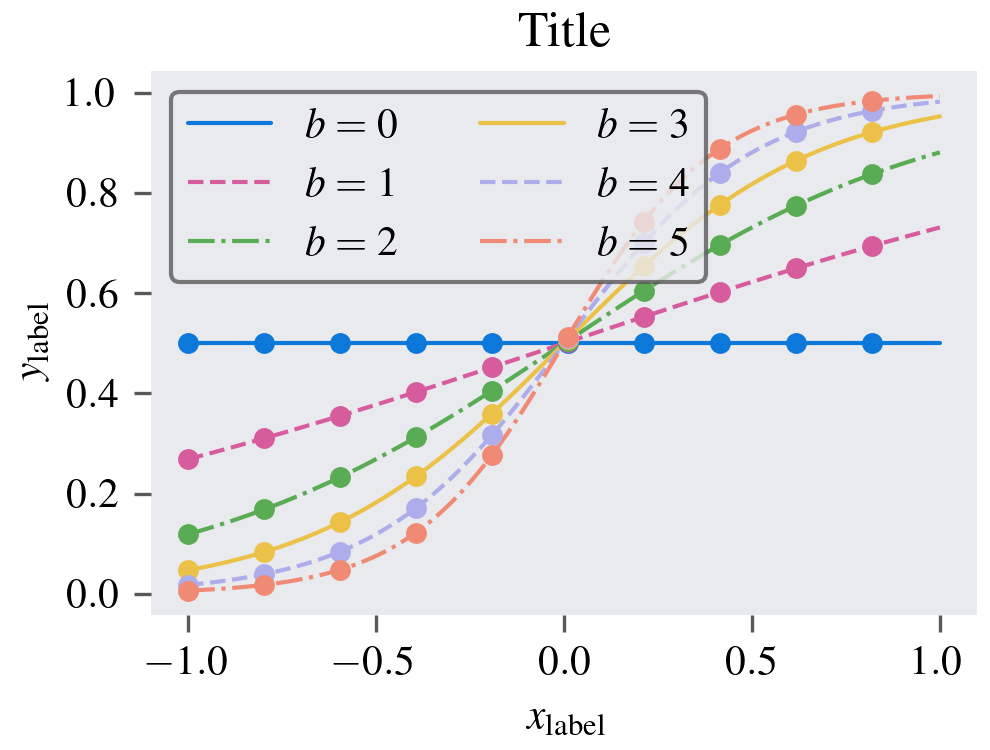
\includegraphics{example-figure}
    \caption{Example caption}
\end{figure}

\section{Method}\label{sec:method}


\subsection{The model}\label{sec:model}

A radial mode frequency is some function of radial order,
\(\nu_{n,l=0} = f(n)\) where \(f\) can be described by a Gaussian process,
%
\begin{equation}
    f(\bm n) \sim \mathcal{GP}\left[m(\bm n), k(\bm n, \bm n')\right],
\end{equation}
%
for array \(\bm n\) with some mean function, \(m(\bm n)\) and kernel function,
\(k(\bm n, \bm n')\).

The mean function comprises a background frequency as a function of \(n\),
\(f_\bkg(n)\), and the glitches due to the second ionisation of helium,
\(\delta_\helium(\nu)\) and base of the convective zone
\(\delta_\bcz(\nu_\bkg)\),
%
\begin{equation}
    m(n) = f_\bkg(n) + \delta_\helium(\nu_\bkg) +
    \delta_\bcz(\nu_\bkg),
\end{equation}
%
where \(\nu_\bkg = f_\bkg(n)\). For the background, we adopt the
asymptotic approximation to first order in \(n\),
%
\begin{equation}
    f_\bkg(n) = \Delta\nu (n + \epsilon),
\end{equation}
%
where \(\Delta\nu\) is the large frequency separation and \(\epsilon\) is some
offset. We define the small change in mode frequency caused by the second
ionisation of helium, \(\delta\nu_\helium = \delta_\helium(\nu)\) as,
%
\begin{equation}
    \delta_\helium(\nu) = a_\helium \nu e^{- b_\helium \nu^2}
    \sin\left( 2 \pi \tau_\helium \nu + \phi_\helium \right),
\end{equation}
%
where \(a_\helium\) is the frequency-dependent amplitude and \(b_\helium\)
relates to the acoustic width of the glitch. We define the small change in
frequency due to the base of the convective zone,
\(\delta\nu_\bcz = \delta_\bcz(\nu)\) as,
%
\begin{equation}
    \delta_\bcz(\nu) = \frac{a_\bcz}{\nu^2}
    \sin\left( 2 \pi \tau_\bcz \nu + \phi_\bcz \right),
\end{equation}
%
where \(a_\bcz\) is the frequency-dependent amplitude. For both glitches,
parameters \(\tau\) and \(\phi\) relate to the acoustic depth and phase of
the glitch respectively.

The kernel function describes the covariance between modes at different \(n\).
We expect consecutive modes to correlate more strongly than modes further
apart. Therefore, we adopt the squared-exponential (or radial basis) kernel
function,
%
\begin{equation}
    k(\bm n, \bm n') = \sigma^2
    \exp\left(- \frac{\| \bm n - \bm n' \|^2}{2\lambda^2}\right),
\end{equation}
%
where \(\sigma^2\) is the variance and \(\lambda\) is the length scale.

The model described above comprises 11 parameters,

\begin{equation}
    \bm\theta = [\Delta\nu, \epsilon, a_\helium, b_\helium, \tau_\helium,
    \phi_\helium, a_\bcz, \tau_\bcz, \phi_\bcz, \sigma^2, \lambda].
\end{equation}

Using Bayes' theorem, we write the posterior probability density function for
the model given some observation of radial mode frequencies \(\bm\nu_n\),
%
\begin{equation}
    p(\bm\theta \mid \bm\nu_n) \propto p(\bm\theta) \,
    p(\bm\nu_n \mid \bm\theta),
\end{equation}
%
where \(\Pi(\bm\theta)\) is the a priori probability of the model and
\(\mathcal{L}(\bm\nu_n \mid \bm\theta)\) is the likelihood of the data given the
model.


\subsection{The prior}\label{sec:prior}

The prior for the model can be separated into a product of the priors for each
individual parameter,
%
\begin{equation}
    p(\bm\theta) = \prod_{i=0}^{10} p(\theta_i).
\end{equation}
%
In the following sections we write our choice of prior for each of
\(\theta_i\).


\subsubsection{Background parameters}\label{sec:bkg-params}

The prior for \(\Delta\nu\) is provided as the location and scale of a
normal distribution, \(\Delta\nu \sim \mathcal{N}(\mu_{\Delta\nu},
\sigma_{\Delta\nu})\). The prior for \(\epsilon\) is chosen to be a log-normal
distribution, \(\epsilon \sim \ln\mathcal{N}(\ln(1.4), 0.4)\).


\subsubsection{Glitch parameters}\label{sec:glitch-params}

The glitch parameters' priors must convey at least two things; the first is
that the glitch amplitudes are approximately \SIrange{0.1}{1.0}{\micro\hertz},
and the second is that the acoustic depths are in physically sensible places.
The former comes from reviewing previous measurements of the glitches in the
literature and can be enforced by inspecting the sensibility of a grid of
glitch amplitude parameters as a function of \(\nu_\mathrm{max}\) (see
Appendix \ldots) The latter is less straightforward to determine, and will be
defined later in this section.

\begin{itemize}
    \item Stellar model grid
    \item Extract acoustic depths
    \item Fit Gaussian mixture to \((\log\nu_\mathrm{max}, T_\mathrm{eff},
          \log\tau_\helium, \log\tau_\bcz)\)
    \item Sample from the conditional distribution of \((\log\tau_\helium,
          \log\tau_\bcz)\) given \((\log\nu_\mathrm{max}, T_\mathrm{eff})\)
    \item This gives the prior for \((\log\tau_\helium, \log\tau_\bcz)\)
\end{itemize}


\subsubsection{Kernel parameters}\label{sec:kernel-params}

We chose to fix the kernel parameters to \(\lambda = 5.0\) and \(\sigma^2 =
0.1 \, \mu_{\Delta\nu}\). \todo{Explain why these values.} The length scale ensures that the
GP does not fit to the glitch, and reflects the typical scale of curvature of
the radial mode frequencies with respect to \(n\). The variance is fixed at
\SI{10}{\percent} of \(\Delta\nu\) which corresponds to the approximate
amplitude of the mode curvature.


\subsubsection{Average amplitude}\label{sec:avg-amp}

The average amplitude of the glitches has been used in previous work as a proxy
for the helium abundance in the star. The average amplitude between frequencies
\(x\) and \(y\) is,
%
\begin{equation}
    \langle A \rangle = \frac{
        \int_{x}^{y} A(\nu) \, \dd \nu
    }{
        \int_{x}^{y} \dd \nu
    }
\end{equation}
%
where \(A(\nu)\) is the amplitude of the glitch at frequency \(\nu\). We derive
this for the helium glitch,
%
\begin{equation}
    \langle A_\helium \rangle = \frac{
        a_\helium \left(
        e^{- b_\helium \, x}
        - e^{- b_\helium \, y}
        \right)
    }{2 b_\helium (y - x)},
\end{equation}
%
and BCZ glitch,
%
\begin{equation}
    \langle A_\bcz \rangle
    = \frac{a_\bcz}{x \, y}.
\end{equation}
%
We expect the average amplitude of the helium glitch to be greater than that of
the convective zone glitch most of the time. \todo{Explain why this is.} To
encode this knowledge into the prior, we introduce the parameter for the
logarithm of the ratio between the average amplitudes of the two glitches.
\(\log r_A = \log \langle A_\helium \rangle - \log \langle A_\bcz \rangle\).
%
\begin{equation}
    \log r_A \sim \mathcal{N}(0.6, 0.3).
\end{equation}
%
The mean is chosen such that the mean lies where
\(\langle A_\helium \rangle = 4 \langle A_\bcz \rangle\). The variance is
chosen such that \(\langle A_\helium \rangle < \langle A_\bcz \rangle\) and
\(\langle A_\helium \rangle > 16 \langle A_\bcz \rangle\) \SI{5}{\percent} of
the time.

\subsection{The likelihood}

The GP likelihood of function for the true frequency \(\bm \nu_n = f(\bm n)\)
given \(\bm\theta\) is a normal distribution,
%
\begin{equation}
    \bm \nu_n \mid \bm\theta \sim
    \mathcal{N}\left[m_\theta(\bm n), k_\theta(\bm n, \bm n)\right].
\end{equation}
%
The likelihood of some noisy observation \(\bm \nu^\mathrm{obs}_n\) of
\(\bm \nu_n\) is,
%
\begin{equation}
    \bm\nu^\mathrm{obs}_n \mid \bm \nu_n
    \sim \mathcal{N}\left[\bm \nu_n, \mathrm{diag}(\bm\sigma_n^2)\right],
\end{equation}
%
where \(\bm\sigma_n^2\) is the array of variances corresponding to
each of \(\bm\nu^\mathrm{obs}_n\), characterising independent, Gaussian noise.

The marginal likelihood of \(\bm\nu^\mathrm{obs}_n\) given the model is thus,
%
\begin{equation}
    \mathcal{L}(\bm\nu^\mathrm{obs}_n \mid \bm\theta)
    = \int p(\bm\nu^\mathrm{obs}_n \mid \bm \nu_n, \bm\theta)
    \, p(\bm \nu_n \mid \bm\theta) \, \dd \bm \nu_n
\end{equation}
%
which given equations above is,
%
\begin{equation}
    \mathcal{L}(\bm\nu^\mathrm{obs}_n \mid \bm\theta) = \mathcal{N}\left[
        \bm\mu_\theta, \bm K_\theta
        + \mathrm{diag}(\bm\sigma_n^2) + \delta
        \right]
\end{equation}
%
where \(\bm\mu_\theta = m_\theta(\bm n)\), \(\bm K_\theta = k_\theta(\bm n, \bm n)\), and
\(\delta = \num{1e-6}\) is some small value to ensure that the covariance is
positive semidefinite.

See C. E. Rasmussen \& C. K. I. Williams for GP conditional
% The conditional distribution for the GP at new radial orders \(\bm\npred\) is
% derived from the joint distribution,
% %
% \begin{equation}
%     \begin{bmatrix}
%         \bm\nu_n\\
%         \bm f_{\npred}
%     \end{bmatrix}
%     \sim \mathcal{N} 
%     \left(
%         \begin{bmatrix}
%             \bm\mu_n\\
%             \bm\mu_{\npred}
%         \end{bmatrix}
%         ,\,
%         \begin{bmatrix}
%             \bm K_n + \bm{\mathcal{I}} \circ (\bm\sigma_n^2 + \delta) & 
%             \bm K_{n, \npred}\\
%             \bm K_{\npred, n} & \bm K_{\npred}
%         \end{bmatrix}
%     \right).
% \end{equation}
%


\section{Results}\label{sec:results}




\subsection{Model stars}\label{sec:model-stars}




\subsection{Sun-as-a-star}\label{sec:sun}




\subsection{\num{16} Cygni}\label{sec:16cyg}




\subsection{KIC \num[group-digits=false]{4448777}}\label{sec:boeing}



%% IMPORTANT! The old "\acknowledgment" command has be depreciated. It was
%% not robust enough to handle our new dual anonymous review requirements and
%% thus been replaced with the acknowledgment environment. If you try to 
%% compile with \acknowledgment you will get an error print to the screen
%% and in the compiled pdf.
\begin{acknowledgments}
    Put acknowledgments here.
\end{acknowledgments}

%% To help institutions obtain information on the effectiveness of their 
%% telescopes the AAS Journals has created a group of keywords for telescope 
%% facilities.
%
%% Following the acknowledgments section, use the following syntax and the
%% \facility{} or \facilities{} macros to list the keywords of facilities used 
%% in the research for the paper.  Each keyword is check against the master 
%% list during copy editing.  Individual instruments can be provided in 
%% parentheses, after the keyword, but they are not verified.

\vspace{5mm}

%% Similar to \facility{}, there is the optional \software command to allow 
%% authors a place to specify which programs were used during the creation of 
%% the manuscript. Authors should list each code and include either a
%% citation or url to the code inside ()s when available.

\software{
    astropy \citep{AstropyCollaboration:2018}, jax \citep{Bradbury:2018},
    jaxns \citep{Albert:2020}, numpy \citep{Harris:2020},
    numpyro \citep{Phan:2019,Bingham:2019}, PBjam \citep{Nielsen:2021}
}

%% Appendix material should be preceded with a single \appendix command.
%% There should be a \section command for each appendix. Mark appendix
%% subsections with the same markup you use in the main body of the paper.

%% Each Appendix (indicated with \section) will be lettered A, B, C, etc.
%% The equation counter will reset when it encounters the \appendix
%% command and will number appendix equations (A1), (A2), etc. The
%% Figure and Table counter will not reset.

\appendix

%% For this sample we use BibTeX plus aasjournals.bst to generate the
%% the bibliography. The sample631.bib file was populated from ADS. To
%% get the citations to show in the compiled file do the following:
%%
%% pdflatex sample631.tex
%% bibtext sample631
%% pdflatex sample631.tex
%% pdflatex sample631.tex

\bibliography{main}{}
\bibliographystyle{aasjournal}

%% This command is needed to show the entire author+affiliation list when
%% the collaboration and author truncation commands are used.  It has to
%% go at the end of the manuscript.
%\allauthors

%% Include this line if you are using the \added, \replaced, \deleted
%% commands to see a summary list of all changes at the end of the article.
%\listofchanges

\end{document}

% End of file `sample631.tex'.
